\documentclass{beamer}
\setbeamertemplate{caption}[numbered]
\usepackage{multirow}
\usepackage{fancyhdr}
\usepackage{graphicx}
\graphicspath{{../images/}}
\usepackage{multimedia}
\usepackage{color}
\usepackage{caption}

\usetheme{Berlin}  %{Berlin}{Hannover}{Singapore}{CambridgeUS}

\title{Generative Adversarial Networks for Automatic Image Colorization}
\subtitle{\textbf{Team}: Yet Another Layer - YAL}


\author{Cameron Fabbri, Md Jahidul Islam}

\begin{footnotesize}

\end{footnotesize}


\begin{document}
\date{}
%%%%%%%%%%%%%%%%%%%%%%%%%%%%%%%%%
\begin{frame}
\thispagestyle{empty}
\titlepage
\end{frame}
%%%%%%%%%%%%%%%%%%%%%%%%%%%%%%%%%

\section*{Preliminaries}
%%%%%%%%%%%%%%%%%
\begin{frame}
\frametitle{\textbf{Image Colorization}}

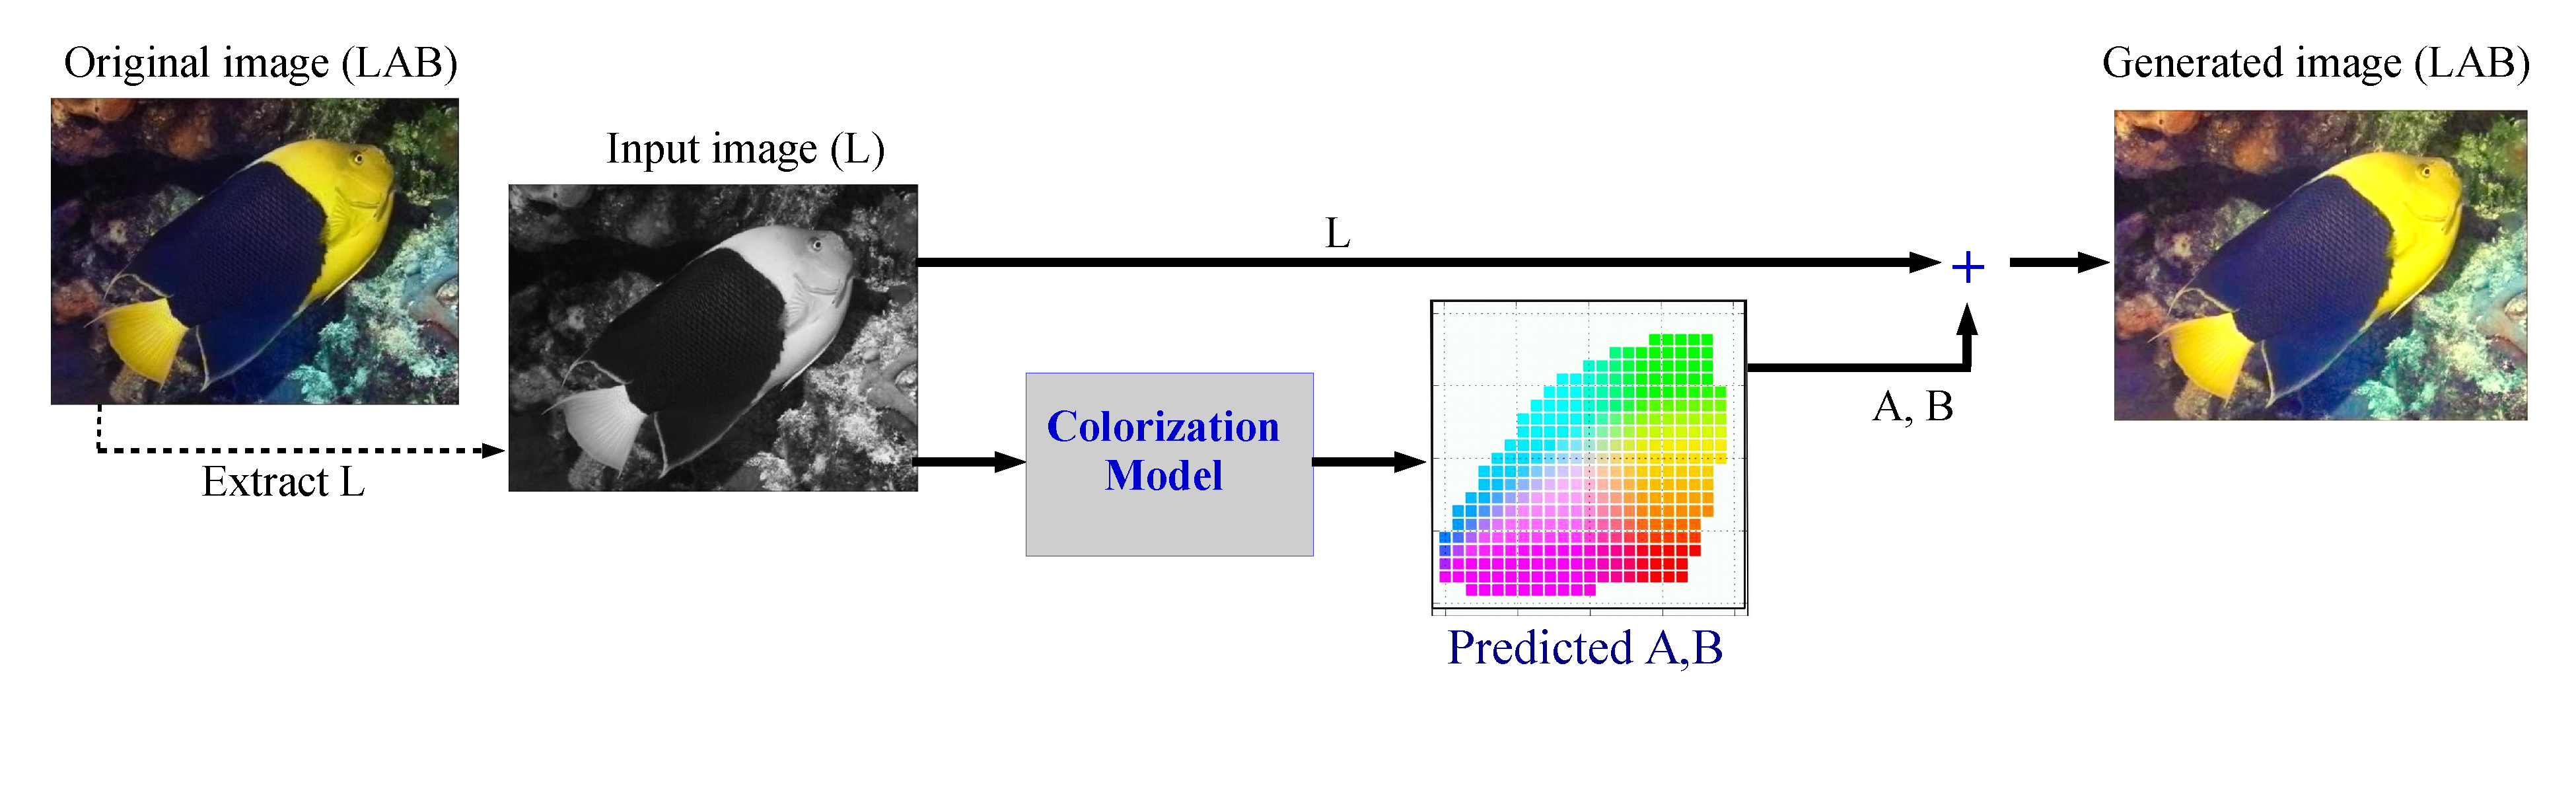
\includegraphics[width=\linewidth]{6.pdf}



\end{frame}

%%%%%%%%%%%%%%%%%% Background
\begin{frame}
\frametitle{\textbf{Background}}
\begin{itemize}
  \item Algorithmic choices:
	\begin{enumerate}[$-$]
	\item  \textbf{Image-to-image translation} 
	\item Classification
	\end{enumerate}
	
	\item Colorspace choices:
  
	\begin{enumerate}[$-$]
	\item  \textbf{LAB}, RGB
	\end{enumerate}
	
	\item Approaches
  
	\begin{enumerate}[$-$]
	\item Classical
	\item Deep learning based
	\begin{enumerate}[$-$]
	  \item Generative models
	  \item \textbf{Adversarial model}
	\end{enumerate}	 
	\end{enumerate}
	
\end{itemize}
\end{frame}
%%%%%%%%%%%%%%%%%%%%%%%

%%%%%%%%%%%%%%%%%%%%%%%
\section*{Classical Models}
\begin{frame}
\frametitle{\textbf{Classical Approaches}}
\framesubtitle{\textbf{Colorization using User-specified Prior [4]}}
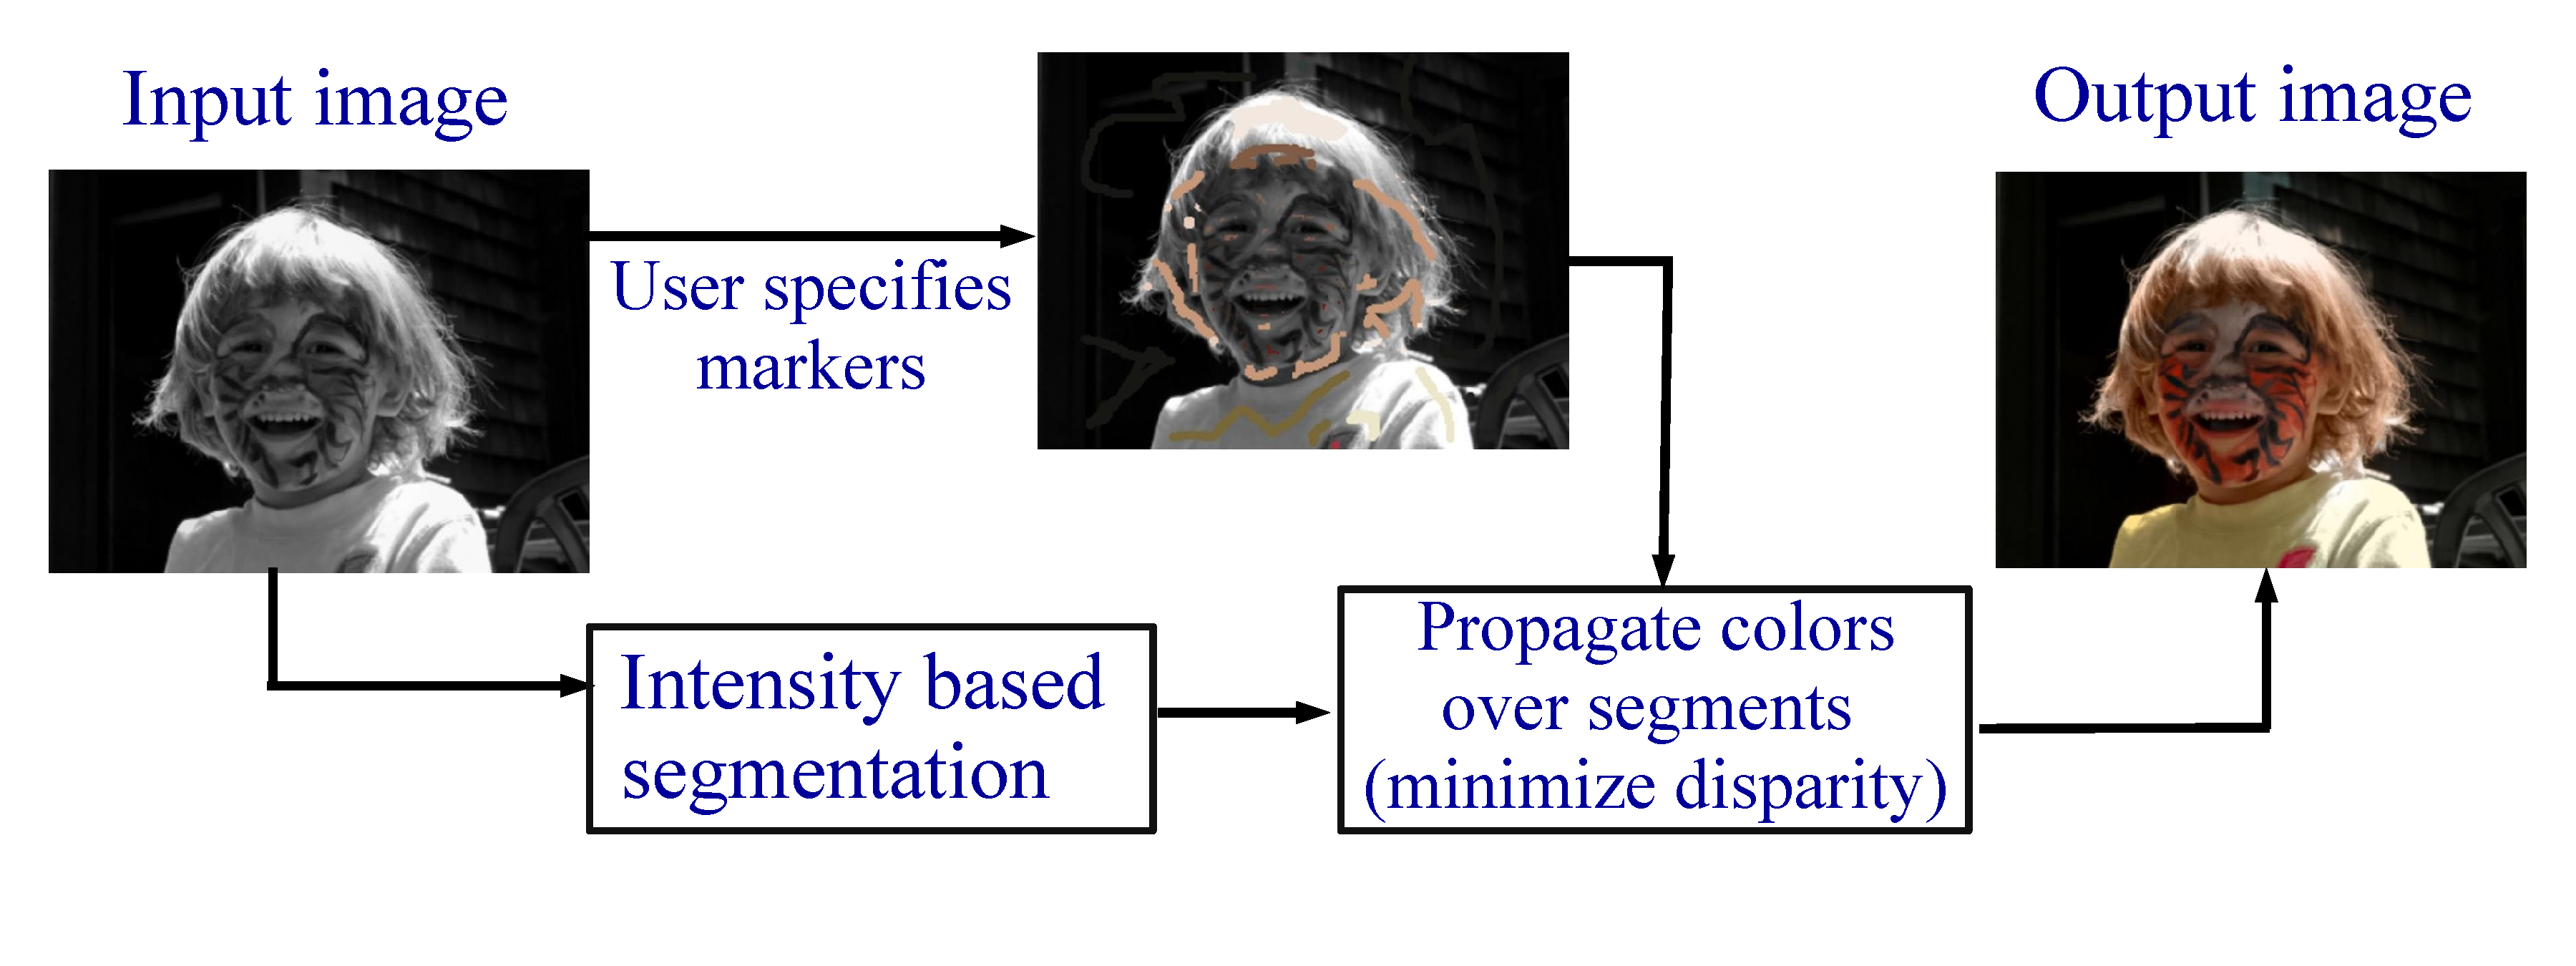
\includegraphics[width=\linewidth]{5.pdf}

\vspace{-3mm}
\begin{table}

\centering
\begin{tabular}{llll}
{\color{blue} \textbf{Pros}} & & & {\color{red} \textbf{Cons}} \\
Fast & & & Not automatic \\
Reliable & & & Not scalable

\end{tabular}
\end{table}

\end{frame}

\begin{frame}
\frametitle{\textbf{Classical Approaches}}
\framesubtitle{\textbf{Colorization using Multi-modal Prediction [5]}}
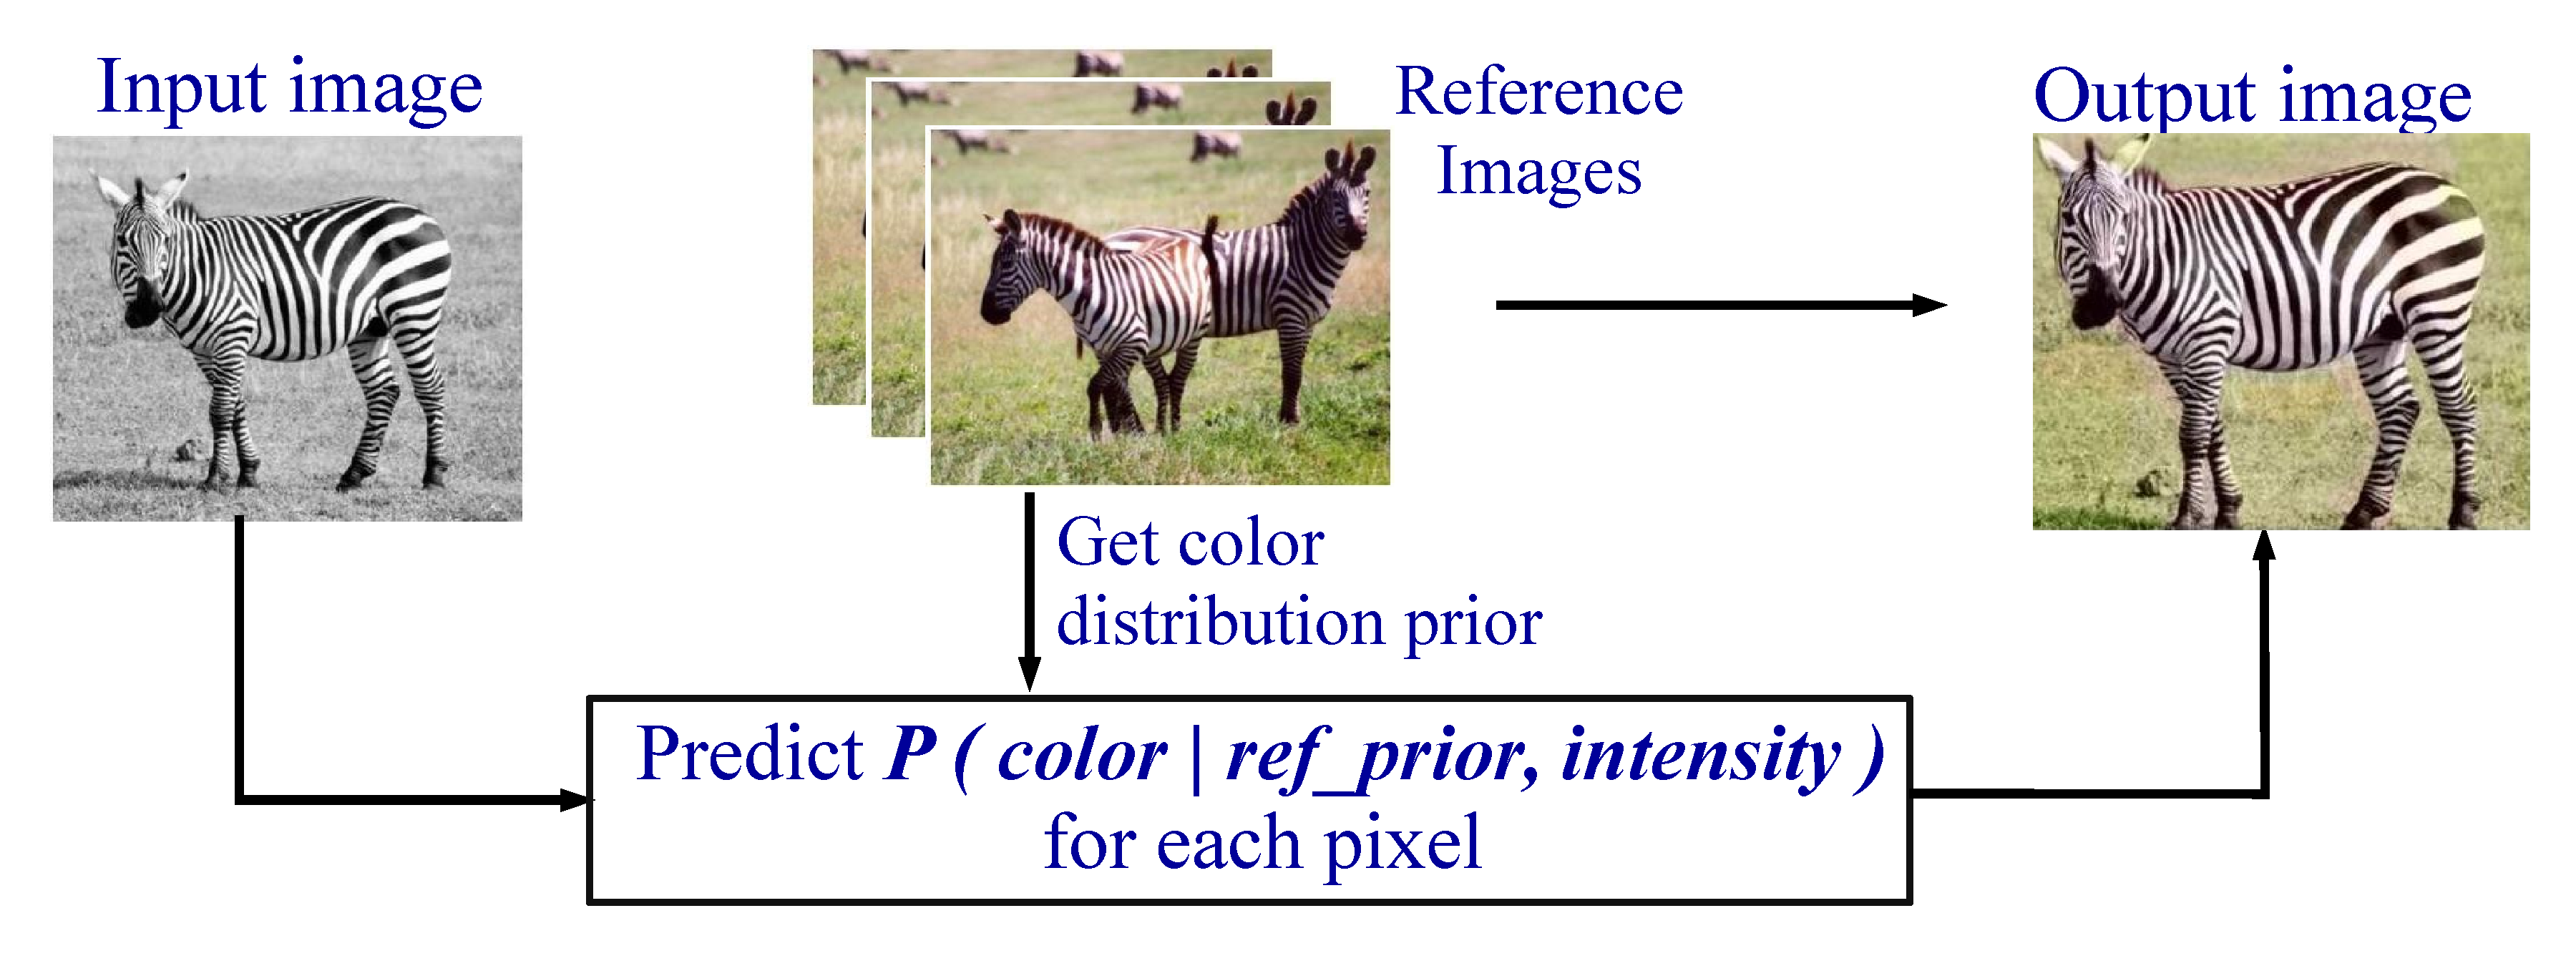
\includegraphics[width=\linewidth]{4.pdf}

\vspace{-5mm}
\begin{table}
\centering
\begin{tabular}{llll}
{\color{blue} \textbf{Pros}} & & & {\color{red} \textbf{Cons}} \\
Automatic & & & Depends heavily on reference prior  \\
Handles multimodality & & & Not practical

\end{tabular}
\end{table}

\end{frame}


\section*{DL: Generative Models}

\begin{frame}
\frametitle{\textbf{Generative Approach}}
\framesubtitle{\textbf{Colorful Image Colorization model [1]}}
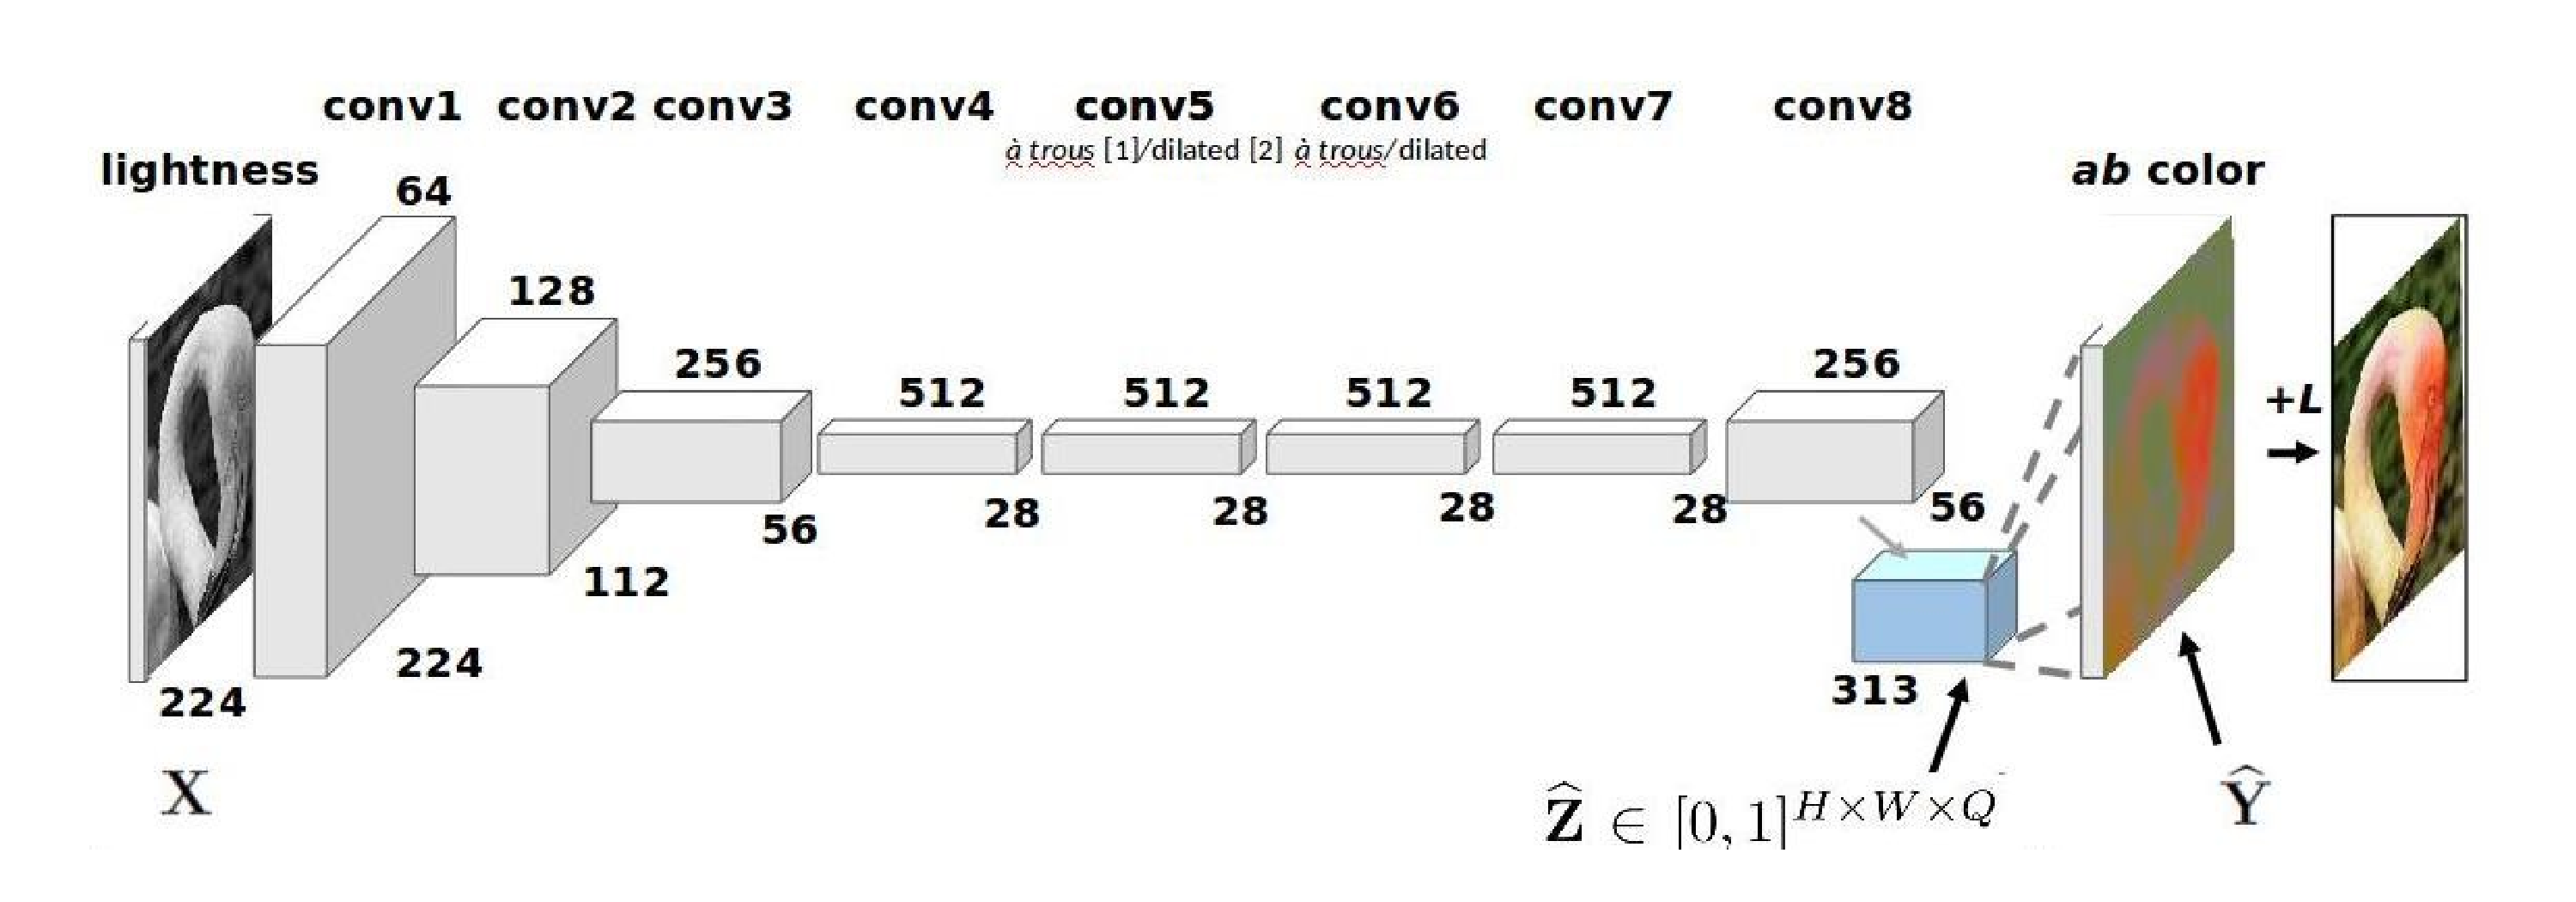
\includegraphics[width=\linewidth]{7.pdf}


\begin{table}
\footnotesize
\centering
\begin{tabular}{|l|l|l|}
\hline 
\textbf{Model Changes} & {\textbf{Original model}}  & {\color{blue} \textbf{Adopted model}} \\
\hline \hline
Output & Classification  Probabilities & {\color{blue} Image}  \\ \hline
Trained on & ImageNet & {\color{blue} CelebA, Places2 }\\ \hline
Implementation & Caffe & {\color{blue}Tensor-flow} \\ \hline

\end{tabular}
\end{table}

\end{frame}

\begin{frame}
\frametitle{\textbf{Results}}
\framesubtitle{\textbf{Colorful Image Colorization model as generator only}}
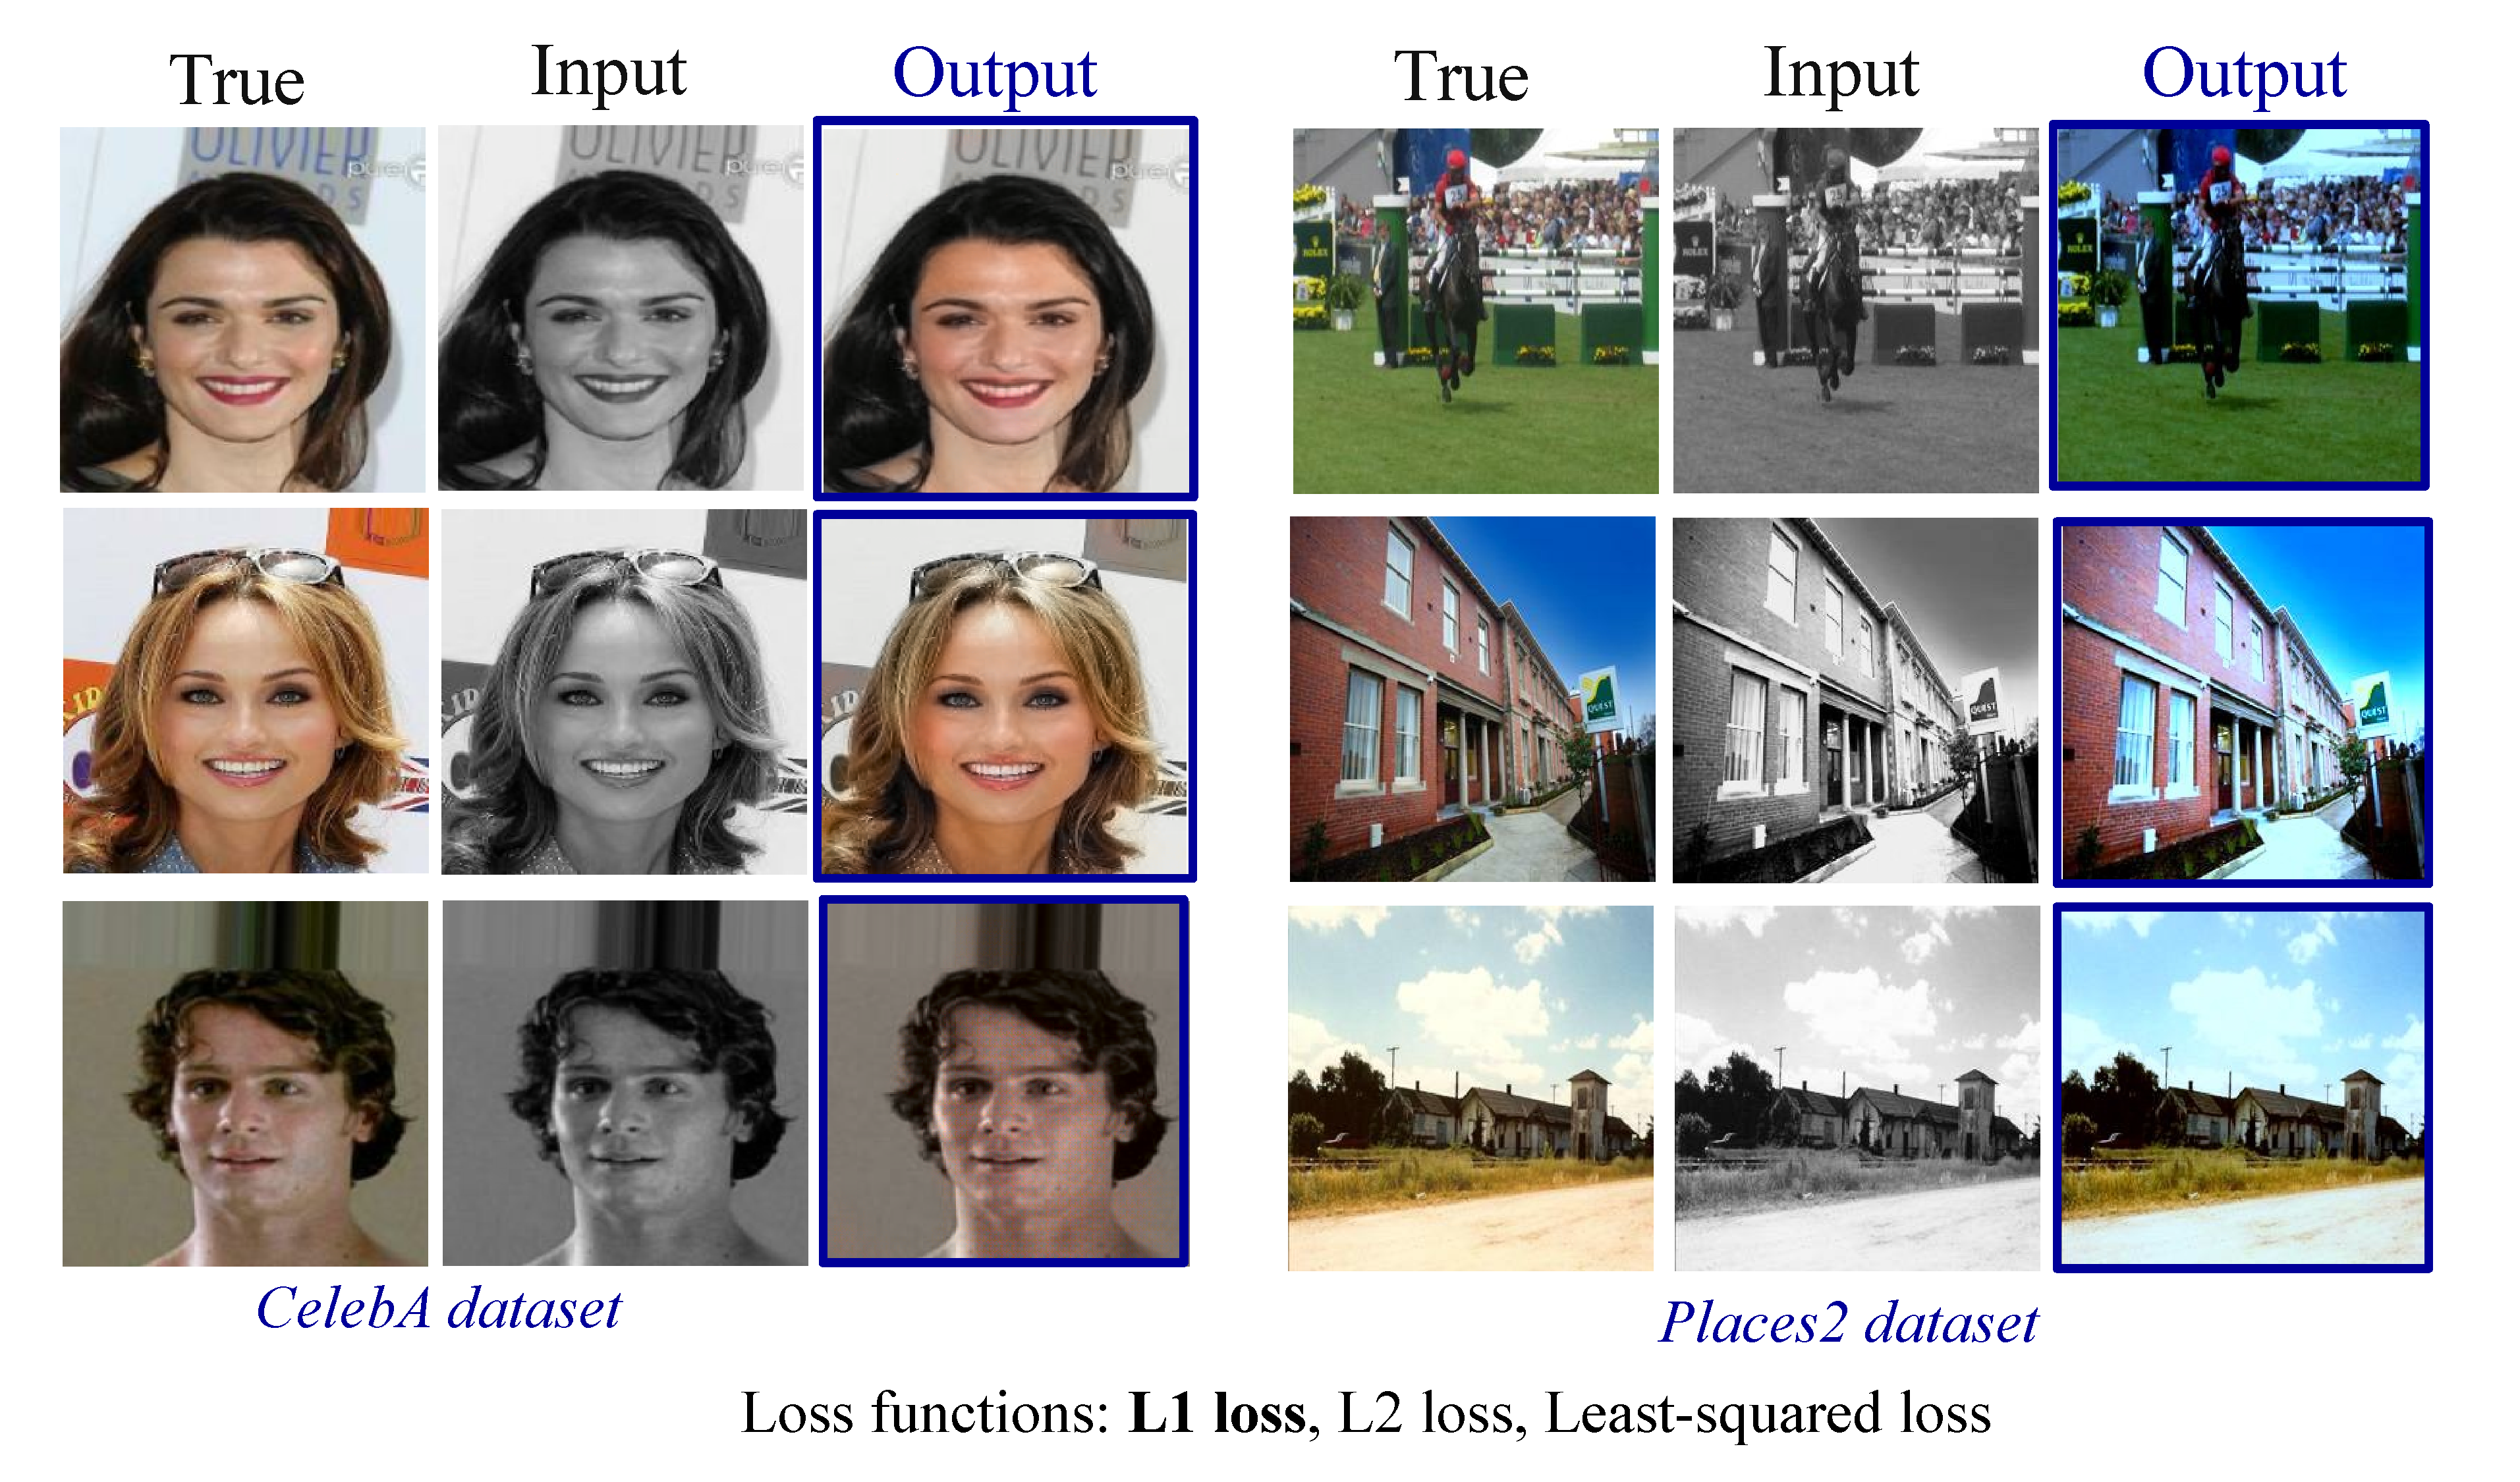
\includegraphics[width=\linewidth]{81.pdf}
\end{frame}

%%%%%%%%%%%%%%%%%%%%%%%%% GANs
\section*{DL: Adversarial Models}
\begin{frame}
\frametitle{\textbf{Results}}
\framesubtitle{\textbf{Colorful Image Colorization model as generator in a GAN}}
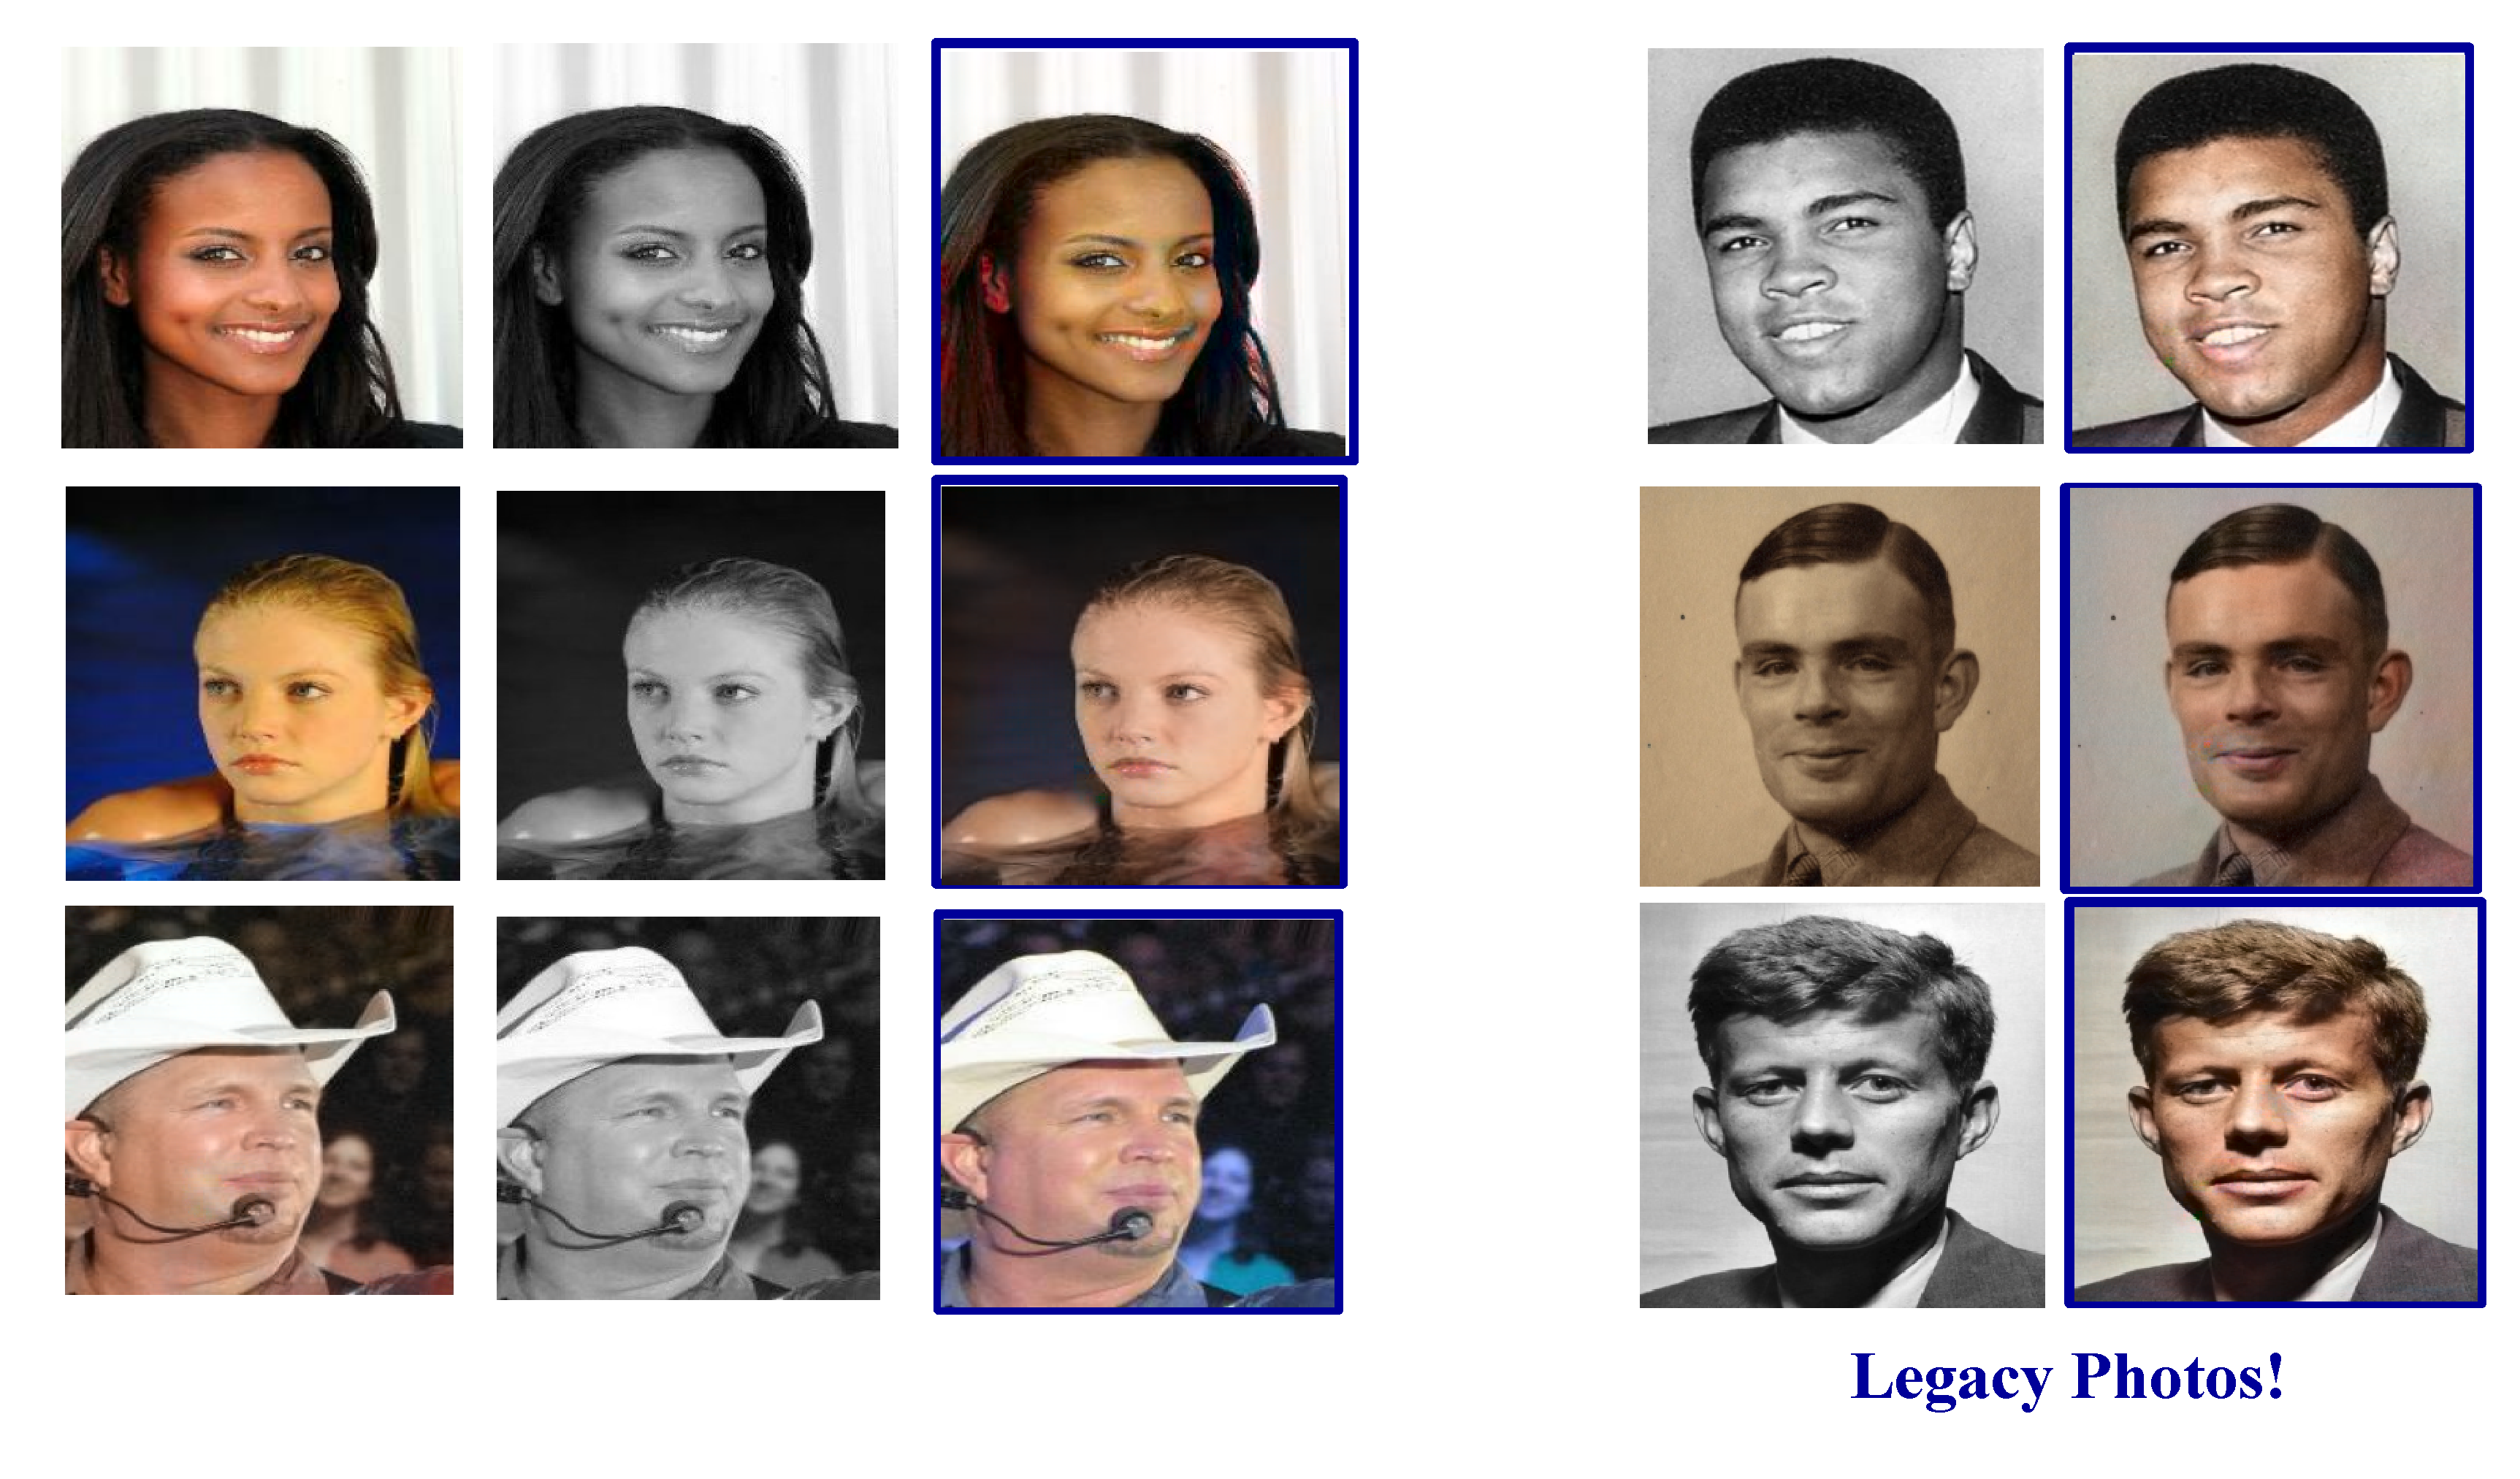
\includegraphics[width=\linewidth]{82.pdf}
\end{frame}




%%%%%%%%%%%%%%%%%%%%%%%%% GANs
\begin{frame}
\frametitle{\textbf{Generative Adversarial Networks (GANs)}}
   \begin{itemize}
      \item Two player minimax game
	   \begin{enumerate}[$-$]
         \item Discriminator \textbf{D}
         \item Generator \textbf{G}
      \hspace{30mm}
\includegraphics[width=0.3in]{noise} \hspace{2mm}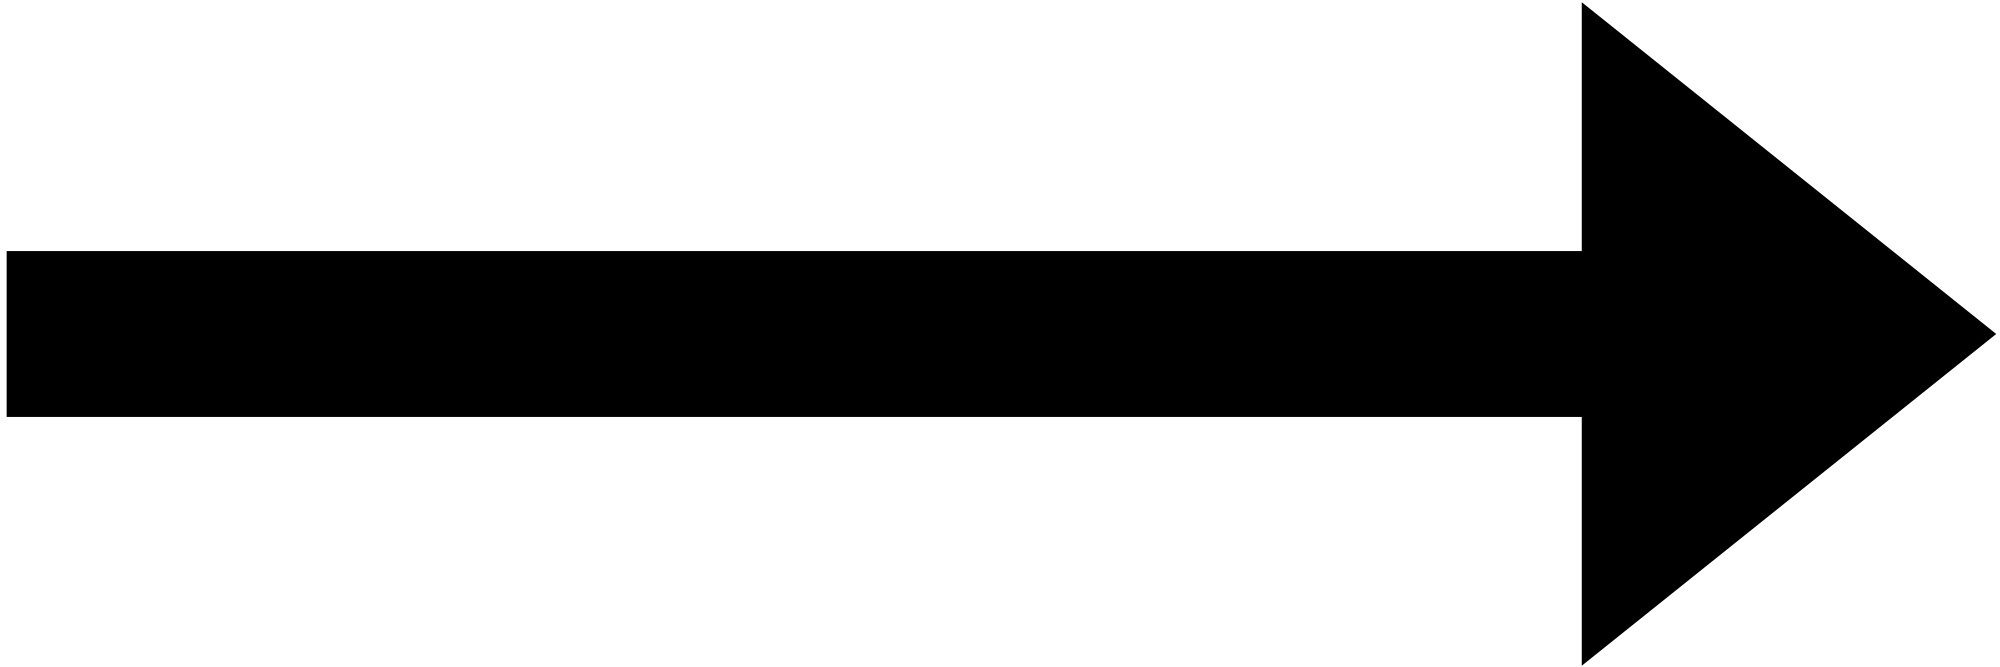
\includegraphics[width=0.5in]{arrow} \hspace{1mm} 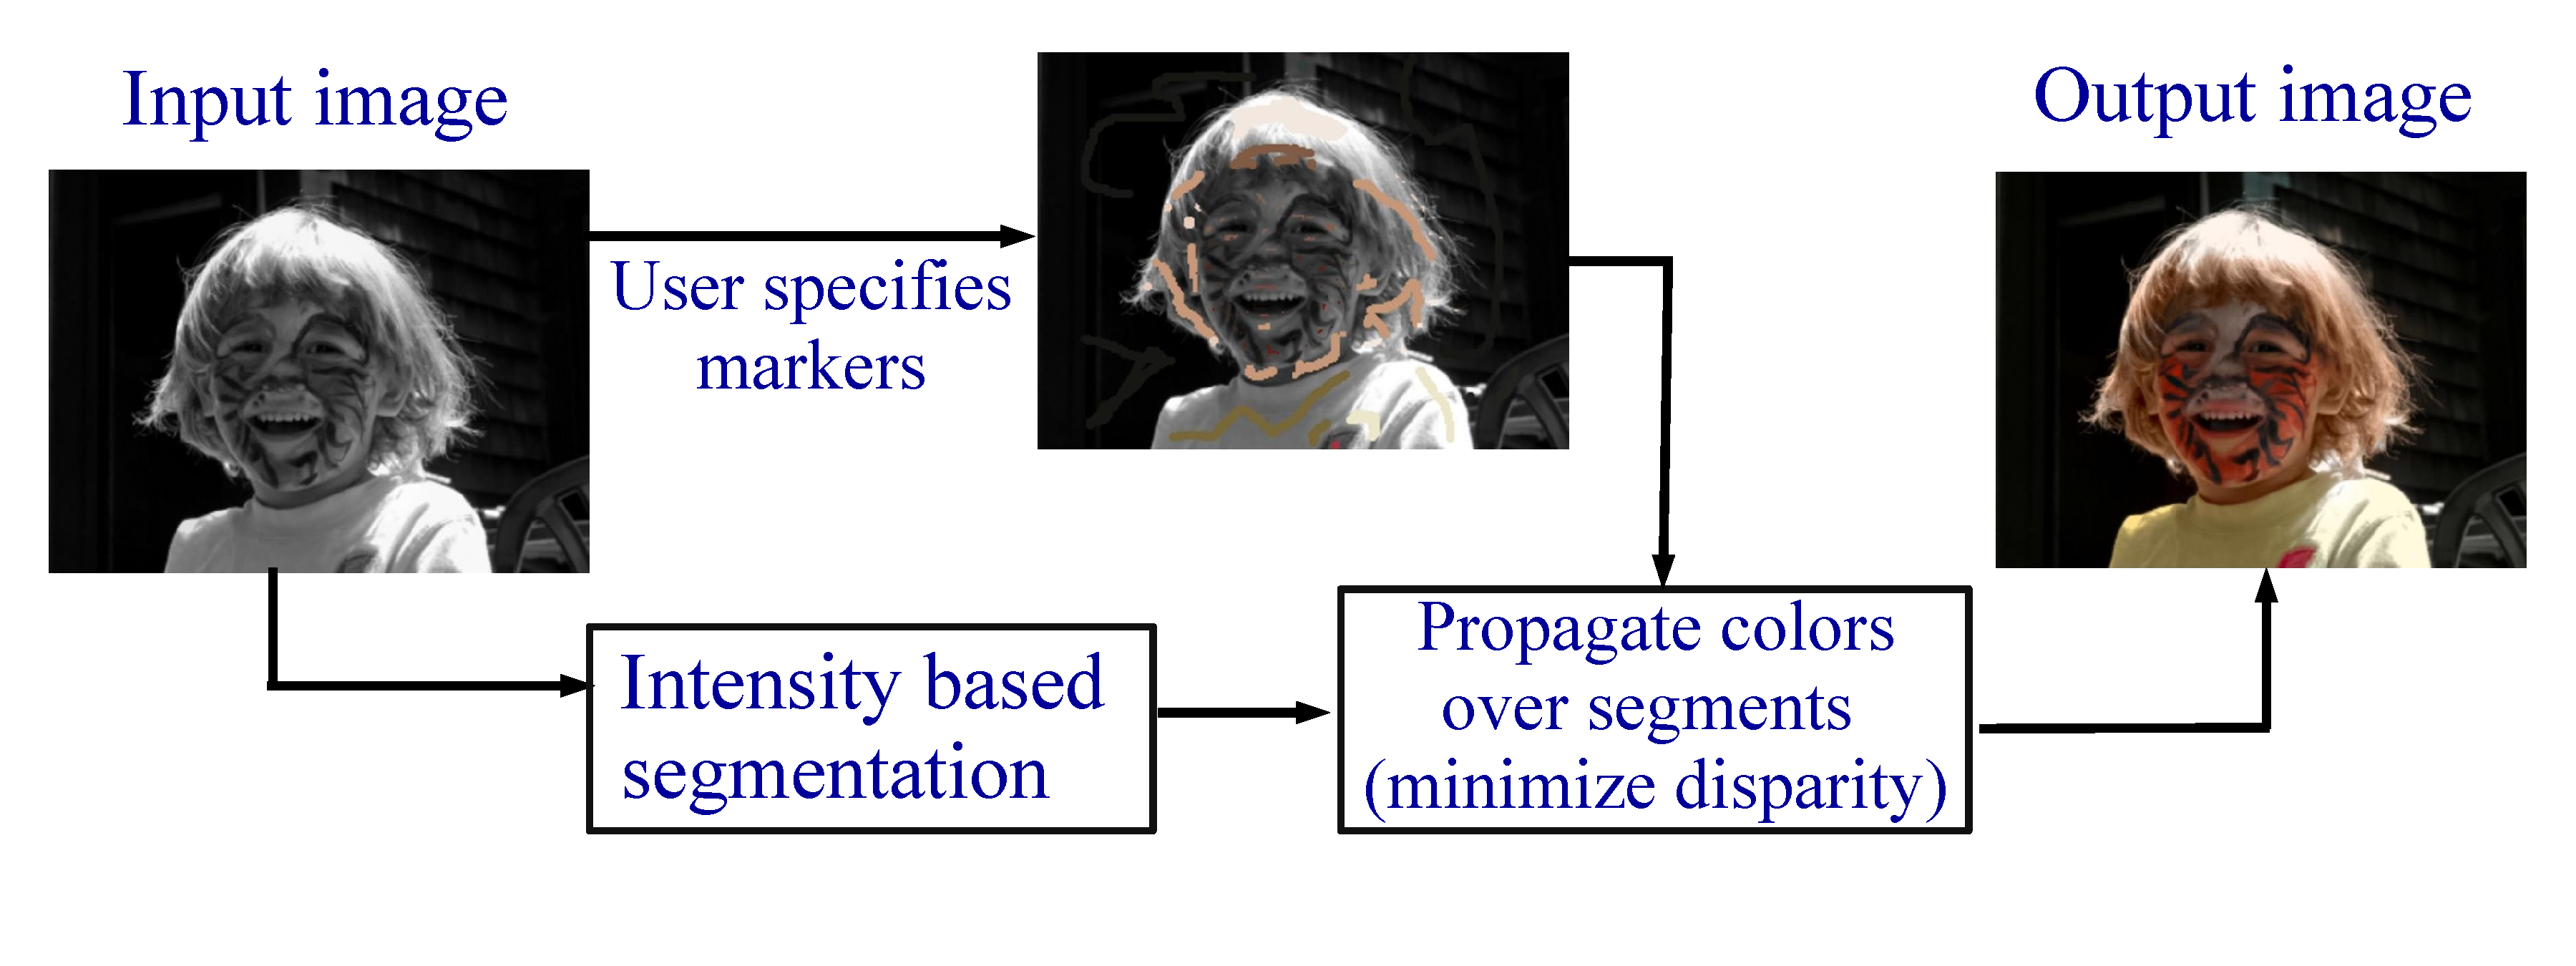
\includegraphics[width=0.3in]{5}
	   \end{enumerate}
      \item D is trained to discriminate between a real image and a generated image
	   \item G is trained to generate an image that will fool D
	   \item Both G and D are neural networks
      \[\min\limits_{G}\max\limits_{D} \mathbb{E}_{x \sim p_{data(x)}} [logD(\textbf{\textit{x}})] + \mathbb{E}_{z \sim p_z(z)}[log(1 - D(G(z)))]\]
	   \item Conditional GANs generate images given conditional information, such as a class label.
   \end{itemize}
\end{frame}
%%%%%%%%%%%%%%%%%%%%%%%

%%%%%%%%%%%%%%%%%% Alternative 
\begin{frame}
\frametitle{\textbf{GAN Variations}}
   \begin{itemize}
      \item Deep Convolutional GANs (DCGANs)
	   \begin{enumerate}[$-$]
         \item Bridge the gap between GANs and Deep Learning
      \end{enumerate}
      \item Least Squares GANs (LSGANs)
	   \begin{enumerate}[$-$]
         \item Use a least squares loss for the discriminator
      \end{enumerate}
      \item Energy-Based GANs (EBGANs)
	   \begin{enumerate}[$-$]
         \item Model the discriminator as an energy function
      \end{enumerate}
      \item Wasserstein GAN (WGAN)
	   \begin{enumerate}[$-$]
         \item Minimizes the Earth Mover distance between two distributions
      \end{enumerate}
   \end{itemize}
\end{frame}


\section*{Results}



%\begin{frame}
%\begin{quote}
%\begin{center}
%\huge{Thank you all !} \\

%\end{center}   
%\end{quote}
%\end{frame}

\begin{frame}
\frametitle{\textbf{References}}
\footnotesize
\begin{enumerate}
\item Richard Zhang, Phillip Isola, and Alexei A Efros. Colorful image colorization. In European Conference on Computer Vision,
pages 649–666. Springer, 2016.
\item Huimin Lu, Yujie Li, and Seiichi Serikawa. Underwater image enhancement using guided trigonometric bilateral filter and fast
automatic color correction. In Image Processing (ICIP), 2013 20th IEEE International Conference on, pages 3412–3416. IEEE, 2013.
\item Luz A Torres-Méndez and Gregory Dudek. Color correction of underwater images for aquatic robot inspection. In International
Workshop on Energy Minimization Methods in Computer Vision and Pattern Recognition, pages 60–73. Springer, 2005.



\end{enumerate}
\end{frame}
\end{document}
